

\section{Methodology}

Reports play a crucial role in medical sectors. Technological inventions in the medical sector
are fast-forwarding, and generating reports using AI is increasingly in demand. However, the
challenges are accuracy and reliability. This project aims to ensure reliability in generating
reports using deep learning methods such as CNN models, RAG, and LLM, which will remove
hallucination and implement explainability. The RAG model merged with deep learning methods
will help to reach reliability, improve factual consistency, and improve accuracy in generating
reports. The Software Development Life Cycle (SDLC) system is followed to build the project
through iterative development, testing, and refinement of individual system components. The
development of the proposed system is described below.

% ─────────────────────────────────────────────────────────────────────────────
\subsection{Requirement Analysis}

In requirement analysis the whole website's required features and functionalities are discussed.
This process consists of problem analysis, literature review, and requirement specification.

\begin{itemize}
    \item \textbf{Problem Analysis:} To detect diseases such as pneumonia, emphysema, and
    pleural effusion, chest X-rays are required. As report generation with precision needs
    expertise, this model is going to assist a radiologist to achieve quality reports.

    \item \textbf{Literature Review Findings:} For chest X-ray analysis, CNN-based models are
    effective, and to learn from X-ray images, DenseNet121 works efficiently. RAG also
    provides improved output using its features in decision making.

    \item \textbf{Requirement Specification:} The system shall include:
    \begin{enumerate}
        \item Upload chest X-ray image
        \item Preprocess images through CNN model for analysis
        \item CNN model like DenseNet121 will extract features from the image
        \item The embeddings and metadata will be stored in ChromaDB
        \item Similar historical cases will be retrieved using RAG properties
        \item The retrieved image reports and contextual information will be displayed
        \item Integration of LLM will generate reports
    \end{enumerate}
\end{itemize}

% ─────────────────────────────────────────────────────────────────────────────
\subsection{System Architecture}

The system architecture includes a website, CNN model DenseNet121, ChromaDB as vector
database, a RAG pipeline, and an LLM. Initially the image is uploaded by a user on the website
and then goes through the DenseNet121 model, which extracts high-level visual features;
embeddings are stored within ChromaDB with metadata including disease labels, image
identifiers, and radiology reports. Embeddings of the input image are compared with the stored
embeddings for identifying similar cases. The retrieved images are showcased as evidence of
the report.

\vspace{0.5em}
\noindent\textbf{Proposed Workflow}

\begin{center}
\begin{tabular}{c}
    Chest X-ray Image \\
    $\downarrow$ \\
    DenseNet121 \\
    $\downarrow$ \\
    Feature Embedding \\
    $\downarrow$ \\
    ChromaDB \\
    $\downarrow$ \\
    Retrieved Similar Cases \\
    $\downarrow$ \\
    Augmented Context \\
    $\downarrow$ \\
    Large Language Model \\
    $\downarrow$ \\
    Suggested Radiology Report \\
\end{tabular}
\end{center}

% ─────────────────────────────────────────────────────────────────────────────
\subsection{Development Tools and Technologies}

Python was the main programming language used in the development of the framework. For
image processing, OpenCV was used; for deep learning, PyTorch and TorchVision were used.
ChromaDB was used as the vector database for storing image embeddings, and it also supports
similarity-based retrieval. For data manipulation and numerical computation, Pandas and NumPy
were employed, whereas Matplotlib was used for visualisation and exploratory analysis.
Development and experimentation were conducted using Google Colab and VS Code.

\vspace{1em}
\begin{table}[H]
    \centering
    \caption{Development Tools and Technologies}
    \label{tab:tools}
    \begin{tabular}{ll}
        \toprule
        \textbf{Category} & \textbf{Technology} \\
        \midrule
        Programming Language      & Python \\
        Deep Learning Framework   & PyTorch \\
        CNN Architecture          & DenseNet121 / ViT \\
        Image Processing          & OpenCV, TorchVision \\
        Data Analysis             & Pandas, NumPy \\
        Visualization             & Matplotlib, GRAD-CAM \\
        Vector Database           & ChromaDB \\
        Development Environment   & Google Colab, Visual Studio Code \\
        Future RAG Integration    & LangChain, Large Language Models \\
        \bottomrule
    \end{tabular}
\end{table}

Image analysis, feature embedding, similarity retrieval, and future report production are the
four main parts of the suggested system. To extract significant visual features from chest X-ray
images, the image analysis component makes use of DenseNet121. Important radiographic
qualities are captured by transforming these features into numerical embeddings.

The created embeddings and related metadata --- such as radiology reports and disease labels ---
are kept in ChromaDB. To find clinically similar past cases, query embeddings are compared to
stored embeddings during retrieval. Retrieved reports offer contextual information that could
help medical professionals analyse images.

Future RAG integration is supported by the architecture. In further stages of development, a
Large Language Model will be fed retrieved reports and accompanying medical documents to
provide structured radiology report recommendations.

% ─────────────────────────────────────────────────────────────────────────────
\subsection{Web Application Design}

The whole system is integrated with a web application to ensure flexible use as a Clinical
Supporting Tool by medical practitioners.
\begin{figure}[H]
    \centering
    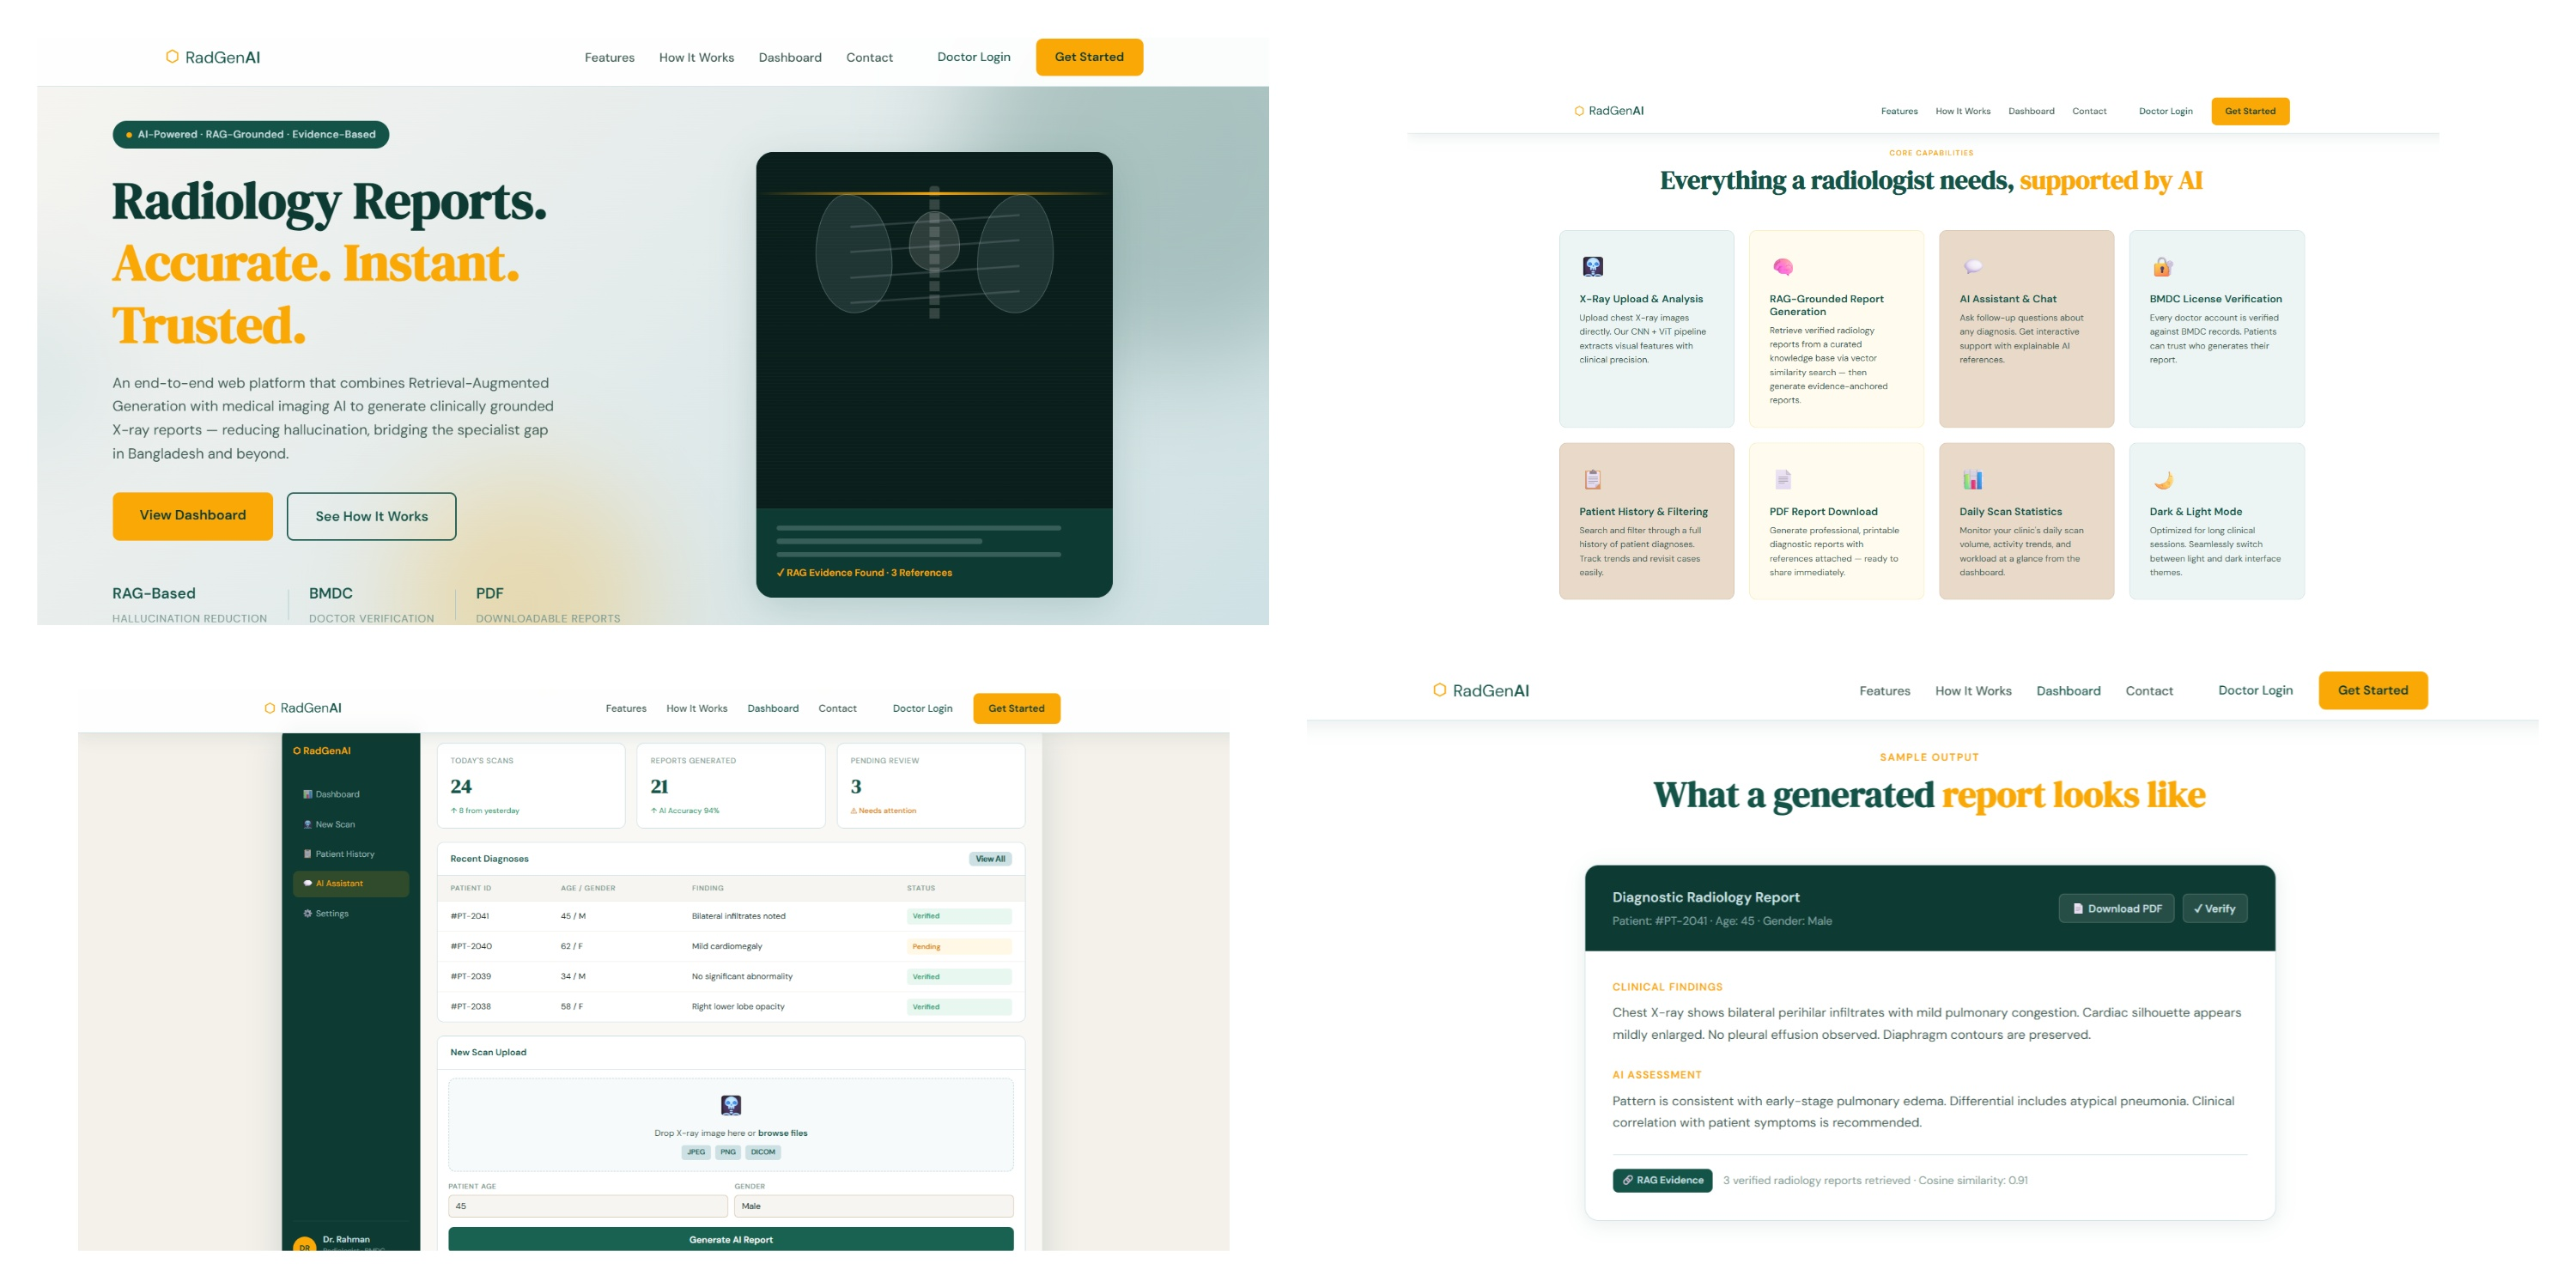
\includegraphics[width=0.8\textwidth]{image4.jpg} 
    \caption{ User Interface (UI) of the radiology report generation web application.}
    \label{fig:system_architecture}
\end{figure}

\subsubsection*{Frontend Design}

The frontend component was developed using React.js. To ensure optimisation of the frontend
it needs to operate fast, which React helps to achieve; the website also needs upgrades and
monitoring, so React is suitable for its component-based architecture.

The frontend functionalities are:
\begin{itemize}
    \item User authentication
    \item BMDC verification
    \item Patient information entry
    \item Chest X-ray image upload
    \item Retrieval result visualisation
    \item Diagnostic history management
\end{itemize}

The interface is designed to provide a simple and intuitive workflow that enables healthcare
professionals to interact efficiently with the system.

\subsubsection*{Backend Design}

The codebase models we have run are mostly Python-based. For compatibility we use FastAPI
as the backend framework, which will help us navigate our work better.

Backend operations are:
\begin{itemize}
    \item Receiving uploaded images
    \item Image preprocessing
    \item DenseNet121 inference
    \item Embedding generation
    \item ChromaDB retrieval
    \item Retrieval result delivery
\end{itemize}

\subsubsection*{Database Layer}

This project uses MongoDB as its database, as it is easier and more flexible to use. As the
database contains confidential information, it is reliable in terms of security. In this database
patient records are managed, such as patient details, past history of diagnosis, relevant
metadata, and user accounts for verification



The rest of the work is ongoing, following the SDLC work plan.

% ============================================================================
\section{Dataset}
% ============================================================================

\subsection{Dataset Description}

The performance of any artificial intelligence system heavily depends on the quality of the
dataset used for training. In this project, chest X-rays and reports were collected from a
publicly available medical dataset from Indiana University. This contains both normal and
abnormal chest radiographs accompanied by their diagnostic reports, but did not contain any
disease labels, which were labelled manually.

The dataset includes multiple disease categories encountered in clinical practice. These
categories include Normal reports, Pneumonia, Cardiomegaly, Pleural Effusion, Pneumothorax,
Emphysema, Fibrosis, Atelectasis, Bronchitis, Granuloma, Degenerative Changes, Healed
Fracture, and Normal Cases. All images were associated with diagnostic labels, which allowed
the model to learn disease-specific visual patterns.

The IU Chest X-Ray dataset was selected because it had both images and radiology reports.
The images were divided into four folders based on their size. There are 7,265 images and
radiology reports. These reports form the knowledge base of the Retrieval-Augmented
Generation (RAG) system. During retrieval, reports of the same type with the highest
similarity are searched and supplied to the Large Language Model for improving factual
consistency of report generation.

% ─────────────────────────────────────────────────────────────────────────────
\subsection{Preliminary Data Analysis}

Understanding the characteristics of a dataset is important when working with it to train a
model. Here we analyse the dataset by checking null values, disease category and ratio, image
projection distribution, and report length.

Initially the dataset consisted of 7,625 unique images, but we created a subset consisting of
the first 1,000 chest X-rays belonging to 12 diseases.

\vspace{1em}
\begin{table}[H]
    \centering
    \caption{Initial Disease Label Distribution (Subset of 1,000 images)}
    \label{tab:disease-dist}
    \begin{tabular}{lc}
        \toprule
        \textbf{Disease Label} & \textbf{Count} \\
        \midrule
        Normal              & 472 \\
        Granuloma           & 110 \\
        Other Abnormality   & 82  \\
        Emphysema           & 64  \\
        Cardiomegaly        & 61  \\
        Degenerative Changes& 61  \\
        Atelectasis         & 53  \\
        Pneumonia           & 35  \\
        Pleural Effusion    & 27  \\
        Healed Fracture     & 17  \\
        Fibrosis            & 14  \\
        Bronchitis          & 4   \\
        \bottomrule
    \end{tabular}
\end{table}

The distribution showed a significant imbalance, so we manually cleaned the dataset and
removed the Normal category, as it was affecting the whole model output. We then
re-categorised the dataset by setting a minimum limit of 60 reports per class. The resulting
dataset consists of six diseases: Normal, Granuloma, Emphysema, Cardiomegaly,
Degenerative Changes, and Other Abnormalities.

The projection distribution showed the presence of both frontal and lateral images and their
frequencies. Variability in report size and clinical depth was shown by report length analysis.
Some reports included diagnostic impressions, while others described radiographic findings in
greater detail. Because it offers greater clinical context for similar case retrieval, this diversity
is advantageous for retrieval-based applications.

% ─────────────────────────────────────────────────────────────────────────────
\subsection{Data Preprocessing}

Initially, all chest X-ray images were fixed to input dimensions compatible with DenseNet121.
We converted X-ray images into tensor format of $224 \times 224$ pixels and normalised them
using ImageNet statistics. Fixing the image dimensions ensured efficient batch processing
during model training. Normalisation helped improve gradient stability.

Image quality verification was performed to filter out bad, corrupted, and duplicated images,
which were then excluded from the dataset. Diagnostic labels were assigned manually using
medical documents and reports and organised in a structured way suitable for supervised
learning. The cleaned reports were then segmented into retrievable text chunks used for vector
database storage.

All these preprocessing procedures improved the quality of the dataset. After preprocessing,
the dataset was divided into training, validation, and testing sets to measure performance and
accuracy.

% ============================================================================
\section{Design (Model) Specification}
% ============================================================================

\subsection{DenseNet121 Disease Classification Model}

We selected DenseNet121 as our primary neural network architecture for disease
classification and feature extraction. DenseNet is part of the family of densely connected
CNNs in which each layer receives feature maps from all preceding layers. The speciality of
this design is that it promotes feature reuse, improves gradient propagation, and reduces the
number of trainable parameters. Unlike other CNN architectures, DenseNet121 uses a densely
connected structure in which every layer receives feature maps from all preceding layers
within the same dense block and passes its own output forward to all subsequent layers.

% ── HOW TO ADD THIS IMAGE ─────────────────────────────────────────────────────
% IMAGE: Figure 4.1 — DenseNet121 Dense Connectivity Pattern diagram
%   1. In Overleaf, click the "Upload" button (top-left, looks like an arrow pointing up).
%   2. Upload your image file (e.g., densenet_connectivity.png or figure4_1.png).
%   3. If you want to organise images in a folder, create a folder called "images" in
%      Overleaf, upload there, and change the filename below to "images/densenet_connectivity.png".
%   4. Replace "densenet_connectivity.png" below with your actual filename.
% ─────────────────────────────────────────────────────────────────────────────
\begin{figure}[H]
    \centering
    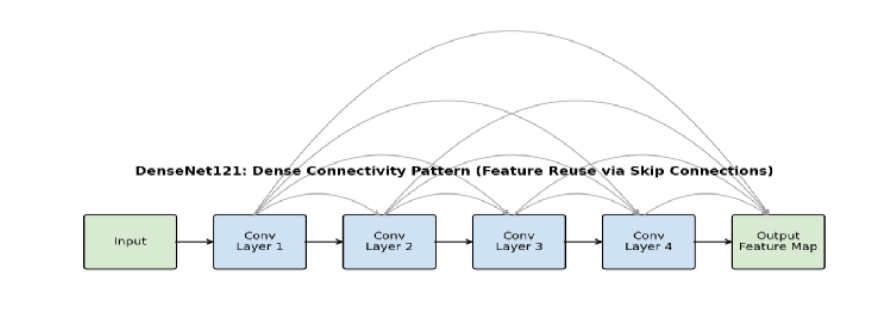
\includegraphics[width=0.75\textwidth]{images/image1.png}
    \caption{Conceptual illustration of dense connectivity within a DenseNet121 dense block,
    where feature maps from earlier layers are concatenated and used by later layers.}
    \label{fig:densenet}
\end{figure}

This connectivity pattern gives several architectural advantages that make DenseNet121
particularly suitable for medical image analysis tasks such as chest X-ray classification.

The model first receives a preprocessed chest X-ray image as input and processes it through
multiple dense blocks and transition layers. During training, DenseNet121 learns hierarchical
visual representations from low-level anatomical structures to high-level disease-specific
abnormalities.

Compared to architectures like VGG16 and ResNet50, DenseNet121 shows greater performance
in medical imaging applications because of its efficient utilisation of feature information. The
architecture effectively captures subtle radiological findings such as pulmonary infiltrates,
pleural abnormalities, and cardiothoracic enlargement. The final classification layer was
designed and modified to predict the disease category relevant to the dataset. During
inference, the model generates a probability score for every disease class. The highest
confidence predictions are utilised in the Retrieval-Augmented Generation framework.

Beyond disease prediction, one feature layer of DenseNet121 acts as a high-dimensional
visual embedding representation of the chest X-ray image. These embeddings are critical for
similarity retrieval within the ChromaDB vector database.

\vspace{1em}
\begin{table}[H]
    \centering
    \caption{Comparison of CNN architectures considered for the disease prediction module.}
    \label{tab:cnn-comparison}
    \begin{tabular}{p{2.8cm} p{5.5cm} p{5.5cm}}
        \toprule
        \textbf{Model} & \textbf{Advantages} & \textbf{Limitations} \\
        \midrule
        VGG16
            & Simple and uniform architecture; well documented and easy to implement.
            & Very large parameter count, leading to high memory usage and slower training. \\
        \addlinespace
        ResNet50
            & Strong feature learning through residual connections and good baseline performance.
            & Higher computational requirements compared to lighter architectures. \\
        \addlinespace
        DenseNet121
            & Excellent feature reuse, strong gradient flow, and proven performance on medical
              imaging tasks.
            & Slightly more inference complexity due to dense feature concatenation. \\
        \bottomrule
    \end{tabular}
\end{table}

% ─────────────────────────────────────────────────────────────────────────────
\subsection{ChromaDB Vector Database}

For Retrieval-Augmented Generation, a vector database is a fundamental component. In this
research ChromaDB was used as our vector database because of its lightweight architecture,
efficient similarity search capabilities, and seamless integration with Python-based ML
workflows.

The main goal of ChromaDB is to store and retrieve clinically relevant information based on
semantic similarity. Traditional databases perform searches using structured fields and text
matching, whereas vector databases retrieve information by comparing numerical
representations of data.

The knowledge base indexed in ChromaDB is constructed from four categories of source
material:

\begin{enumerate}
    \item \textbf{IU X-Ray radiology reports}, which give real examples of how findings and
    impressions are written for chest X-ray cases.
    \item \textbf{Disease description documents}, which give structured clinical descriptions of
    each disease category supported by the system.
    \item \textbf{Radiology reporting templates}, which provide the structure of a report.
    \item \textbf{Clinical reporting guidelines}, covering standard terminology and reporting
    conventions used by radiologists.
\end{enumerate}

During the preprocessing stage, each of these documents is cleaned and split into smaller text
chunks suitable for embedding. Each chunk is converted into a fixed-length numerical vector
using an embedding model, and the resulting vectors are stored in ChromaDB along with
metadata identifying the source document and disease category. This indexing process creates
the searchable knowledge base which the retrieval module queries at inference time.

When a new chest X-ray image is uploaded, the DenseNet121 model generates a corresponding
feature embedding. This embedding is submitted as a query vector to ChromaDB, which then
performs similarity matching and identifies the most relevant historical cases using
nearest-neighbour search algorithms.

The retrieval process follows four major stages:

\begin{enumerate}
    \item \textbf{Embedding Generation:} The feature representation produced by DenseNet121
    for the uploaded chest X-ray, together with the predicted disease label, is converted into a
    query embedding.
    \item \textbf{Vector Storage:} This query embedding is evaluated by comparing it to the
    pre-computed embeddings stored in ChromaDB.
    \item \textbf{Similarity Search:} ChromaDB locates the most closely related cases and
    documents by executing a nearest-neighbour search based on cosine similarity.
    \item \textbf{Context Retrieval:} The most relevant documents are retrieved and passed
    forward to the context augmentation stage.
\end{enumerate}

The retrieved results contain past chest X-ray reports, disease descriptions, and clinically
relevant examples. These documents collectively form the data supplied to the Large Language
Model.

% ─────────────────────────────────────────────────────────────────────────────
\subsection{Retrieval-Augmented Generation (RAG)}

A major limitation of Large Language Models is their tendency to generate hallucinated
information. Although these models are capable of producing fluent text, they may sometimes
generate unsupported medical findings that could compromise diagnostic reliability.

To mitigate this risk, a Retrieval-Augmented Generation (RAG) pipeline was integrated into
the proposed system. In this pipeline the LLM is not asked to generate a report from scratch.
Instead, before generation begins, the system retrieves a small set of clinically relevant
documents --- such as previously verified radiology reports for visually similar cases,
structured disease descriptions, and standard radiology reporting templates --- and supplies
these documents to the LLM as additional context. The LLM is then prompted to base its
output on this retrieved evidence rather than relying solely on its internal parameters.

The implemented RAG pipeline begins after disease prediction and feature embedding
generation. Once a query embedding is produced, ChromaDB retrieves the most relevant
historical reports and disease-related references. These retrieved documents are combined with
the predicted disease labels generated by DenseNet121.

The proposed retrieval design provides several benefits:

\begin{enumerate}
    \item Reduction of hallucinated clinical statements, since the model is grounded in
    retrieved, verified text rather than free generation alone.
    \item Improved factual accuracy, because the disease labels predicted by DenseNet121 are
    cross-referenced against retrieved disease descriptions before being expressed as output.
    \item Better alignment with historical radiology reporting practices.
    \item Evidence-supported outputs, allowing each generated statement in the report to be
    traced back to a retrieved source document.
    \item Better clinical consistency, as the retrieved radiology templates help standardise the
    structure and terminology used across generated reports.
    \item Increased trustworthiness for healthcare professionals.
\end{enumerate}

Unlike normal report generation systems, the proposed design provides contextual support for
every generated report, improving the credibility of AI-assisted diagnostic recommendations.

% ── HOW TO ADD THIS IMAGE ─────────────────────────────────────────────────────
% IMAGE: Figure 4.2 — RAG Pipeline diagram
%   1. Upload your image to Overleaf (e.g., rag_pipeline.png).
%   2. Replace "rag_pipeline.png" below with your actual filename.
% ─────────────────────────────────────────────────────────────────────────────
\begin{figure}[H]
    \centering
    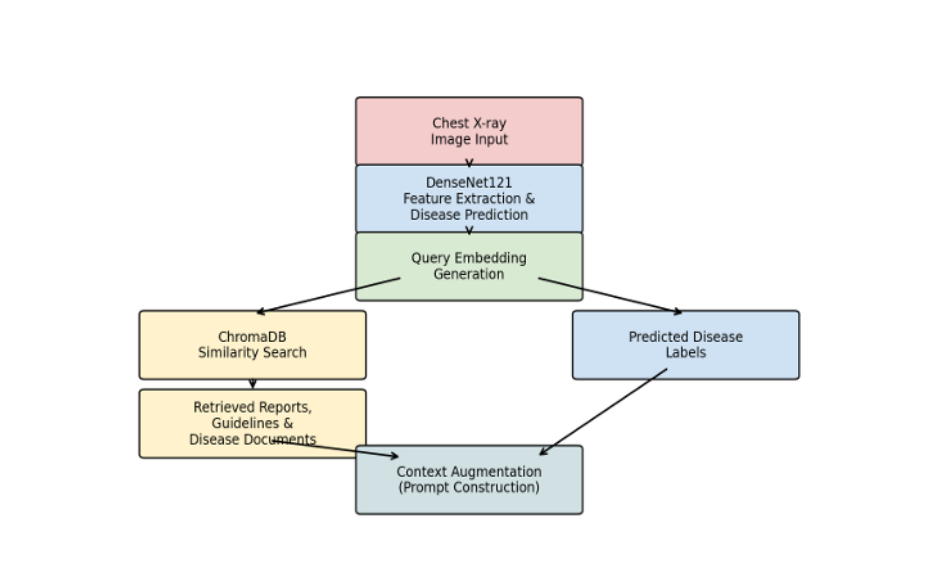
\includegraphics[width=0.80\textwidth]{images/image2.png}
    \caption{Retrieval-Augmented Generation Pipeline used in the system.}
    \label{fig:rag}
\end{figure}

% ─────────────────────────────────────────────────────────────────────────────
\subsection{Large Language Model (LLM)}

The Large Language Model (LLM) acts as the final report generation component of the
proposed system architecture.

The input provided to the language model includes:

\begin{enumerate}
    \item Predicted disease labels
    \item Retrieved radiology reports
    \item Structured disease descriptions
    \item Clinical reporting templates
\end{enumerate}

The extracted information acts as a knowledge base that steers the Large Language Model
while generating reports.

The generated report structure follows formats commonly used in clinical practice, consisting
of:

\begin{enumerate}
    \item \textbf{Findings} --- radiological characteristics.
    \item \textbf{Impression} --- a summary of the most important abnormalities.
    \item \textbf{Diagnostic Summary} --- an overall picture of the whole case.
\end{enumerate}

% ─────────────────────────────────────────────────────────────────────────────
\subsection{Report Generation Flow}

The whole report production workflow is brought about by combining image analysis,
information retrieval, and LLM generation into a single pipeline. When a user or medical
specialist uploads a chest X-ray image through the web application, the whole workflow
process starts.

The uploaded image is prepared for the next stage by preprocessing, resizing, and
normalisation. The refined image is then sent to the DenseNet121 model, which performs
disease classification and feature extraction.

The generated feature embedding is then used to query inside the ChromaDB vector database.
ChromaDB searches and retrieves the most similar cases together with their respective
radiology reports and disease-related information.

The context and disease predictions are combined and sent to the Large Language Model,
which uses this information to create a properly structured radiology report.

The final report is then delivered to the user interface, where professionals can review the
report, provide their opinions, and save it for future reference.

% ── HOW TO ADD THIS IMAGE ─────────────────────────────────────────────────────
% IMAGE: Figure 4.3 — End-to-End Report Generation Workflow diagram
%   1. Upload your image to Overleaf (e.g., report_workflow.png).
%   2. Replace "report_workflow.png" below with your actual filename.
% ─────────────────────────────────────────────────────────────────────────────
\begin{figure}[H]
    \centering
    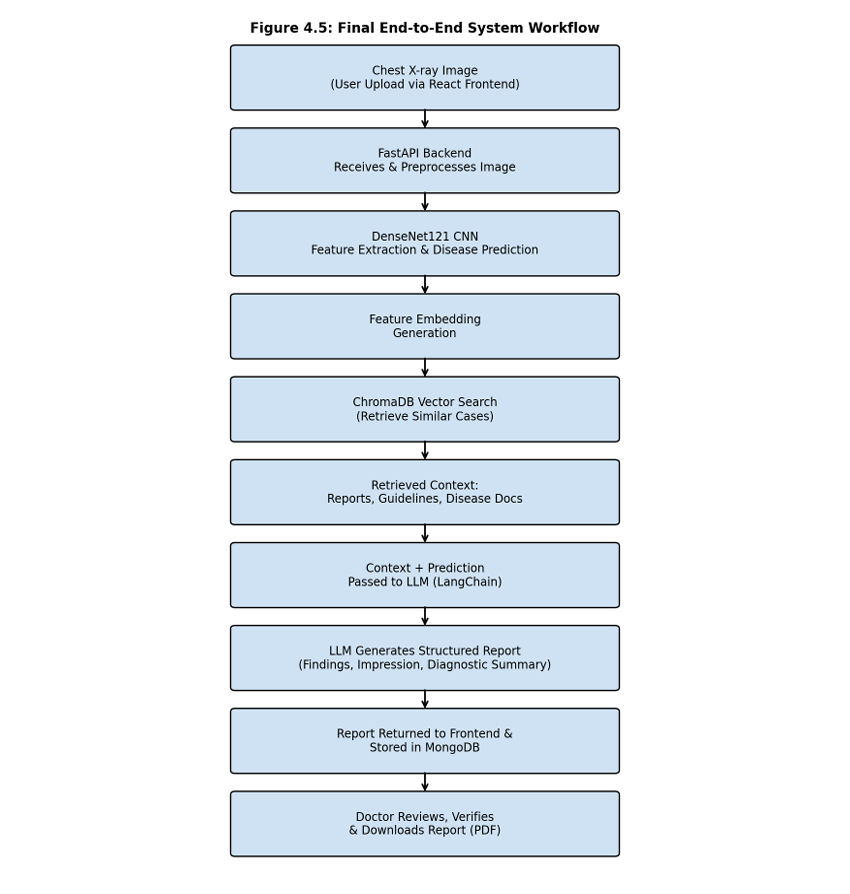
\includegraphics[width=0.65\textwidth]{image3.png} % <-- REPLACE with your filename
    \caption{End-to-End Report Generation Workflow.}
    \label{fig:workflow}
\end{figure}

% ─────────────────────────────────────────────────────────────────────────────
\subsection{System Evaluation Methodology}

\subsubsection*{DenseNet121 Training and Validation Performance}

\begin{table}[H]
\centering
\caption{DenseNet121 Training and Validation Performance}
\label{tab:training}

\small

\begin{tabular}{c c c c c}
\toprule
\textbf{Epoch} &
\textbf{Training Loss} &
\textbf{Training Accuracy (\%)} &
\textbf{Validation Loss} &
\textbf{Validation Accuracy (\%)} \\
\midrule
1 & 1.5529 & 43.03 & 1.3308 & 55.91 \\
2 & 0.9636 & 62.35 & 1.3294 & 54.33 \\
3 & 0.6634 & 86.39 & 1.3391 & 51.97 \\
4 & 0.4203 & 94.45 & 1.4363 & 55.12 \\
\bottomrule
\end{tabular}

\end{table}

\end{figure}
\begin{table}[H]
    \centering
    \caption{Evaluation Metrics}
    \label{tab:metrics}
    \begin{tabular}{lc}
        \toprule
        \textbf{Metric} & \textbf{Value} \\
        \midrule
        Accuracy            & 56\% \\
        Weighted Precision  & 43\% \\
        Weighted Recall     & 56\% \\
        Weighted F1-score   & 44\% \\
        \bottomrule
    \end{tabular}
\end{table}

Only 1,000 reports are labelled out of 7,265 reports, which were used as the sample model
run. Due to the imbalance of the ``Normal'' class, which had 472 entries compared to other
classes like Pneumonia or Pleural Effusion, the model was biased. As a result, when
DenseNet121 was trained over four epochs on the IU Chest X-ray dataset, training performance
varied. Training accuracy improved from 43.03\% in the first epoch to 94.45\% in the fourth,
but validation accuracy remained stable within a maximum of 51.91\%. The gap between
training and validation performance indicates overfitting caused by the imbalanced labelled
dataset. Performance can be improved by labelling all 7,265 reports and removing the class
imbalance.

% ─────────────────────────────────────────────────────────────────────────────
\subsection{Future Improvements and Limitations}

The proposed system demonstrates the effectiveness of combining deep learning, vector
retrieval, and large language models for automated radiology report generation, but several
limitations remain.

First, the current system only focuses on chest X-ray images. Other imaging modalities such
as Computed Tomography (CT), Magnetic Resonance Imaging (MRI), and ultrasound are not
included.

Second, retrieval quality heavily depends on the diversity and quality of the knowledge base
and the selected dataset. Limited coverage of rare diseases may affect retrieval performance
and deteriorate report quality.

Third, the reports generated by this system should only be considered as decision-supporting
recommendations or second opinions for specialists; these are not definitive medical diagnoses.
Clinical validation by specialist professionals is essential.

Future enhancements that can improve this system include:

\begin{enumerate}
    \item Label all 7,265 reports in the dataset and fix the imbalanced data to improve model
    and RAG pipeline accuracy.
    \item Integrate GRAD-CAM explainability.
    \item Compare with Vision Transformer (ViT) architectures.
    \item Expand disease categories and datasets.
    \item Use a cloud-based deployment for nationwide access.
    \item Integrate this system with hospital information systems.
\end{enumerate}

\end{document}